%        File: agree.tex
%     Created: Fri Mar 24 09:00 AM 2017 E
% Last Change: Fri Mar 24 09:00 AM 2017 E
%
% arara: pdflatex: {options: "-draftmode"}
% arara: biber
% arara: pdflatex: {options: "-draftmode"}
% arara: pdflatex: {options: "-file-line-error-style"}
\documentclass[MilwayThesis]{subfiles}

\begin{document}
Crucial to both label theory in general and its application in this thesis, is syntactic agreement.
The highest XP in a given chain must agree with its sister YP in order to converge, and a subset of functional heads must agree in order to label (\textit{e.g.}, English T$_\varphi$).
In this chapter I will discuss the theory of agreement, as it relates to labeling and show how the version of agree required for labeling avoids an undergeneration issue apparently predicted for predicative adjectives in French-type languages.

Agreement is required in label theory to account for (\textit{e.g.},) Subject-TP structures as in \Next.
\ex. [$_\alpha$ DP$_\varphi$ [$_\beta$ T$_\varphi$ ZP]]

The labels of both $\alpha$ and $\beta$ depend on agreement between the subject and T.
Since $\alpha$ is a Phrase-Phrase structure, its label will be $\langle\varphi,\varphi\rangle$ provided DP and T agree for $\varphi$.
This agreement also renders $\beta$ labelable, since, prior to agreement, English T$_\varphi$, with an incomplete $\varphi$-set, is too weak to label \parencite{chomsky2013problems}.
Agreement has the effect of strengthening T such that it can label.

To understand how Agree and Label interact, we must first consider what sort of operations they each are abstracting away from their actual implementations.
Both are take syntactic objects as inputs and operate on them iteratively and locally.
This means that labeling a structure like \Last requires labeling all of its substructures (Iterativity) and that labeling $\beta$ depends solely on the properties of $\beta$ (Locality).
The same, then, is true for Agree, which iteratively considers each substructure and performs agreement is the conditions for agreement are met.

Because labeling is sometimes contingent on agreement, the calculation of the latter must precede that of the former.
Assuming both Agree and Label occur after narrow syntax and before transfer to CI, this leaves us with two possibilities for ordering the two operations.
Either (i) individual iterations of Agree and Label are ordered with respect to each other forming a single Agree+Label cycle or (ii) Agree and Label each has its own cycle, and those cycles are ordered with respect to each other.
To decide between these two alternatives we can consider how Agree and Label interact with other components of grammar, specifically the SM and CI interfaces.
By hypothesis, Label feeds interpretation at CI but not at SM.
Agree, on the other hand, feeds Label and interpretation at SM.
This asymmetry points to the second alternative, where narrow syntax feeds an Agree cycle, which feeds SM interpretation and Label as in \ref{fig:SepCycles}.
The first alternative, in which Agree and Label are bundled into a single cycle as shown in \ref{fig:OneCycle}, predicts that both Label and Agree feed both interfaces, which is not what we seem to see in the data. 
\begin{figure}[h]
  \centering
  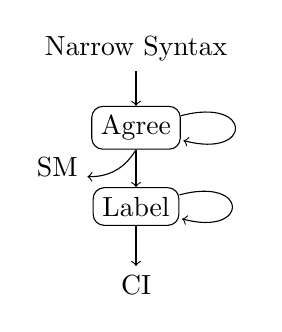
\begin{tikzpicture}
    \node (syn) at (1,3) {Narrow Syntax};
    \node[draw,rounded corners] (agree) at (1,2) {Agree};
    \node[draw,rounded corners] (label) at (1,1) {Label};
    \node (SM) at (0,1.5) {SM};
    \node (CI) at (1,0) {CI};
    \path[->](syn)	edge			(agree)
    (agree)		edge [loop right]	()
	   (agree.south)	edge			(label)
			  edge [bend left]	(SM)
	  (label)		edge [loop right]	()
			  edge			(CI);
  \end{tikzpicture}
  \caption{Agree and Label as separate cycles}
  \label{fig:SepCycles}
\end{figure}
\begin{figure}[h]
  \centering
  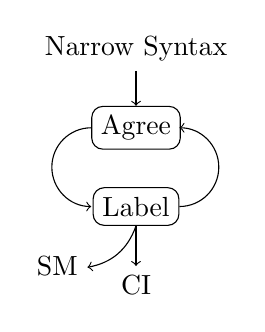
\begin{tikzpicture}
    \node (syn) at (1,3) {Narrow Syntax};
    \node[draw,rounded corners] (agree) at (1,2) {Agree};
    \node[draw,rounded corners] (label) at (1,1) {Label};
    \node (SM) at (0,0.25) {SM};
    \node (CI) at (1,0) {CI};
    \path[->](syn)edge 		(agree)
    (label.south)	edge		(CI)
    (label.south)	edge[bend left]	(SM);
    \draw[->] (label.east) arc(270:450:0.5cm);
    \draw[->] (agree.west) arc(90:270:0.5cm);
  \end{tikzpicture}
  \caption{Agree and Label bundled in a single cycle}
  \label{fig:OneCycle}
\end{figure}

<+FinishThisThought+>

Separating Agree and Label allows us to fix an apparent undergeneration problem in the account of *resultatives in chapter \ref{sec:deriving}, above.
Specifically, the account offered seems to predict that French disallows adjectives in predicate position as in \Next below.
\exg. Jeanne est grand -e\\
Joan is tall -\textsc{FSg}\\
``Joan is tall''

Indeed, without any further clarifications, the system proposed would bar \Last and similar structures.
Assuming the simplified sructure in \Next, below, for \Last, we expect the small clause $\beta$ and the adjP $\alpha$ to be unlabelable.
\ex. 
\begin{forest}
  nice empty nodes,sn edges,baseline,for tree={
    calign=fixed edge angles,
  calign primary angle=-30,calign secondary angle=70}
  [$\delta$
    [DP$_\varphi$[Jeanne,roof]]
    [$\gamma$
      [T$_\varphi$]
      [$\beta$
	[$\langle$DP$_\varphi\rangle$]
	[$\alpha$
	  [adj$_\varphi$]
	  [\textsc{grand}]
	]
      ]
    ]
  ]
\end{forest}

French \textit{adj} has a single $\varphi$-set, meaning it can only label if it is strengthened by an Agree operation.
If we were to assume that Label and Agree were bundled, we might assume that, just as lower copies are invisible to Label, they are invisible to Agree.
This would mean that movement of the DP \textit{Jeanne} would bleed agreement with \textit{adj}, thus rendering $\alpha$ and $\beta$ unlabelable.
We could save \LLast, by hypothesizing that lower copies are visible to Agree but invisible to label, but this would predict that French generates resultatives, clearly an unwanted result.
This means that the visibility conditions for Agree must be distinct from the visibility conditions for Label.
In the remainder of this section I will discuss the visibility conditions for Agree and show how \LLast can be derived.

To begin, let's compare the two relevant structures: the copular clause in \Next, and the resultative adjunct in \NNext.

\ex. Copular clause\label{fig:cop-clause}
\begin{forest}
  nice empty nodes,sn edges,baseline,for tree={
    calign=fixed edge angles,
  calign primary angle=-30,calign secondary angle=70}
  [$\zeta$
    [C]
    [$\delta$
      [DP$_\varphi$[Jeanne,roof,name=subj]]
      [$\gamma$
	[T$_\varphi$]
	[$\beta$
	  [$\langle$DP$_\varphi\rangle$]
	  [$\alpha$
	    [adj$_\varphi$]
	    [\textsc{grand}]
	  ]
	]
      ]
    ]
  ]
  \draw[thick] ([xshift=-12pt]subj.west) arc(180:130:5cm);
\end{forest}

\ex. Resultative adjunct \label{fig:result-adjunct}
\begin{forest}
  nice empty nodes,sn edges,baseline,for tree={
    calign=fixed edge angles,
    calign primary angle=-30,calign secondary angle=70
  }
  [$\delta$
    [DP$_\varphi$[le m\'etal,roof]]
    [$\gamma$
      [res]
      [$\beta$
	[$\langle$DP$_\varphi\rangle$,name=insitu]
	[$\alpha$
	  [adj]
	  [\textsc{plat}]
	]
      ]
    ]
  ]
  \draw[thick] (insitu.south west) arc(180:130:3cm);
\end{forest}

The most salient difference between the DP chains in \LLast and \Last are that the latter crosses a phase boundary, while the former does not.
This fact, I propose, is relevant for Agree's visibility conditions.
Whether or not a movement chain crosses a phase boundary can be made relevant to Agree if Agree operates not on syntactic objects but on chains.
To see how this would work, I will consider the derivations of \LLast and \Last in turn below.

The copular clause, \ref{fig:cop-clause}, is derived from a small clause ($\beta = \left[ \text{DP,} \left[ \text{adj, }\textsc{grand} \right] \right]$) which merges with a finite T$_\varphi$ to form $\gamma$.
The DP, then, merges with $\gamma$ and C is merged triggering phase operations (Agree, Label, Transfer) on it's complement $\delta$.
Agree takes $\delta$, which contains a full DP chain, and values $\varphi$ features on T and adj with $\varphi$ features of DP.
This has two relevant effects: first, it strengthens T and adj such that they can label, and second it renders the lower copy of DP inactive/invisible for Label.
Label then operates on the output of Agree and successfully sends a labelled phrase marker to CI.
\ex. Agree(\ref{fig:cop-clause})\label{fig:agree-cop-clause}\\
\begin{forest}
  nice empty nodes,sn edges,baseline,for tree={
    calign=fixed edge angles,
    calign primary angle=-30,calign secondary angle=70
  }
  [$\delta$
    [DP$_\varphi$[Jeanne,roof,name=subj]]
    [$\gamma$
      [T$_{\langle\varphi,\varphi\rangle}$]
      [$\beta$
	[\sout{DP$_\varphi$}]
	[$\alpha$
	  [adj$_{\langle\varphi,\varphi\rangle}$]
	  [\textsc{grand}]
	]
      ]
    ]
  ]
\end{forest}

\ex. Label(\ref{fig:agree-cop-clause})
\a. Label($\delta$) = $\langle\varphi,\varphi\rangle$
\b. Label($\gamma$) = T
\b. Label($\beta$) = Label($\alpha$) = adj

Thus, the derivation of a copular clause converges in French.

Next, consider the resultative adjunct in \ref{fig:cop-clause} which does not converge in French.
We start with a small clause 
\end{document}
